\section{Protected rectangular interiors}\label{sec:frames}
The same first-difference principle protects a finite interior when the
reference trajectory never enters it. Here the protected set lies inside a
black frame. We first give the exact shielding and entrance statements, then
prove them with complete-field affine-word certificates. All cells outside the
displayed finite input are white. For this section define
\[
 \tau_{\rm hw}(X)=\min\{t\ge0:\text{the complete future trace from }X_t
                         \text{ is standard P104}\}.
\]
Write $\tau(n,m)=\tau_{\rm hw}(R_{n,m},(0,0),N)$ for a solid rectangle;
this is an entrance time, distinct from the earlier half-plane exit time.
\subsection{Four-layer rectangular shielding}
For positive integers $n,m$, put
\[
 R_{n,m}=[0,n-1]\times[0,m-1]\cap\Z^2.
\]
When $n,m\ge10$, define the deep interior and the four-layer frame by
\[
 I_{n,m}=[4,n-5]\times[4,m-5]\cap\Z^2,
 \qquad G_{n,m}=R_{n,m}\setminus I_{n,m}.
\]
Start the ant at $(0,0)$ facing north.

\begin{theorem}[Shielding and exact entrance]\label{frame:thm:frame}
For every $n,m\ge10$ and every $A\subseteq I_{n,m}$, the complete input $B_A=G_{n,m}\cup A$ has the same infinite head and turn trace as the solid rectangle $R_{n,m}$. No cell of $I_{n,m}$ is ever read. Its first permanent standard entrance time and drift per $104$ updates are given by Table~\ref{frame:tab:four}.
\end{theorem}
\begin{table}[ht]
\centering
\small\begin{tabular}{ccrc}
\toprule
$n$ & $m$ & First permanent entrance $\tau(n,m)$ & Drift \\
\midrule
even & even & $78n+44m+555$ & $(2,2)$ \\
even & odd & $30n+44m+438$ & $(2,-2)$ \\
odd & even & $38n+62m+1538$ & $(-2,2)$ \\
odd & odd & $28n+28m+287$ & $(-2,-2)$ \\
\bottomrule
\end{tabular}
\caption{All four formulas include the full transient. The input pose is fixed at the southwest corner facing north.}\label{frame:tab:four}
\end{table}

\begin{figure}[ht]
\centering
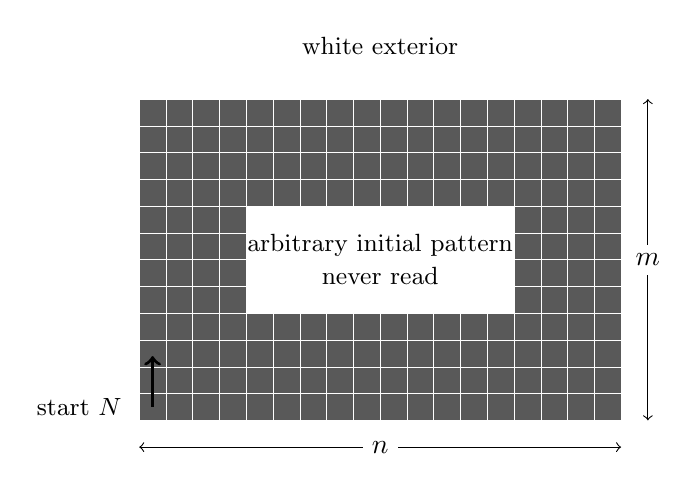
\begin{tikzpicture}[x=0.34cm,y=0.34cm]
\fill[black!65] (0,0) rectangle (18,12);
\fill[white] (4,4) rectangle (14,8);
\draw[step=1,white!35,very thin] (0,0) grid (18,12);
\fill[white] (4.15,4.15) rectangle (13.85,7.85);
\node[align=center] at (9,6) {\small arbitrary initial pattern\\\small never read};
\draw[very thick,->] (0.5,0.5)--(0.5,2.4);
\node[anchor=east] at (-0.3,0.5) {\small start $N$};
\draw[<->] (0,-1)--(18,-1);\node[fill=white] at (9,-1) {$n$};
\draw[<->] (19,0)--(19,12);\node[fill=white] at (19,6) {$m$};
\node at (9,14) {\small white exterior};
\end{tikzpicture}
\caption{The four-layer initial frame. The ant evolves on the full lattice from this initial colouring.}\label{frame:fig:frame}
\end{figure}

For a fixed pair of dimensions, Theorem~\ref{frame:thm:frame} covers exactly $2^{(n-8)(m-8)}$ choices of the interior. More precisely, the complete physical fields satisfy
\begin{equation}\label{frame:eq:field-difference}
 B^A_t\xor B^{A'}_t=A\xor A'\qquad(t\ge0).
\end{equation}
The internal information stays present and unchanged; it is not erased in a reduced simulation.

\begin{proposition}[Sharpness of the common-trace thickness]\label{frame:prop:thickness}
Four is the minimum integer frame thickness that guarantees the common-trace shielding assertion uniformly over the domain $n,m\ge10$.
\end{proposition}
\begin{proof}
Theorem~\ref{frame:thm:frame} gives sufficiency. In the solid $10$-by-$10$ input, the first read of $(3,3)$ occurs at update $1242$ and requests $L$. Removing that one initially black cell preserves the first $1242$ turns and changes the turn at that update to $R$. Both inputs have a black frame of thickness three. The first-read witness is checked by literal vector dynamics in \texttt{controls.py}. It also defeats every smaller thickness, since the same modified cell is then unconstrained.
\end{proof}

\subsection{All solid rectangles and a sharp uniform bound}
Write $\tau(n,m)=\tau_{\rm hw}((R_{n,m},(0,0),\mathrm N))$, including dimensions below ten.

\begin{theorem}[Complete solid-rectangle classification]\label{frame:thm:solid}
Every positive pair $n,m$ has a finite $\tau(n,m)$. Its exact value is specified by four two-parameter affine branches, thirty-six one-parameter affine branches, and a table of $3501$ finite pairs. For all positive $n,m$,
\begin{equation}\label{frame:eq:uniform}
 \tau(n,m)\le242(n+m)+29325.
\end{equation}
The coefficient $242$ is minimal among bounds $\alpha(n+m)+C$ with a fixed finite $C$. At coefficient $242$, the additive constant $29325$ is minimal.
\end{theorem}

Here is the precise partition, including its finite boundary. Table~\ref{frame:tab:four} covers $n,m\ge10$. If $n=i\in\{1,\ldots,9\}$ and $m\ge200$, use the first two formula columns of Appendix~\ref{frame:sec:thin}. If $m=i\in\{1,\ldots,9\}$ and $n\ge200$, use its last two columns. Every remaining pair belongs to
\begin{equation}\label{frame:eq:finitepairs}
 E=\{(n,m):1\le n,m<200,\ \min(n,m)\le9\}.
\end{equation}
These domains are disjoint and exhaustive. The cardinality is $199^2-190^2=3501$. The complete finite table is supplied as the corner rows of \texttt{finite\_report.json}; its check does not infer any untested dimension from a nearby one.

\begin{proof}[Proof of the uniform bound and sharpness, given the certificate leaves]
Each affine branch is verified as an actual infinite trajectory by Section~\ref{frame:sec:verification}. On a thin branch, write the long side as $L=200+p+2a$, where $p\in\{0,1\}$ and $a\ge0$. The exact entrance is $\alpha L+\beta$, with every $\alpha\le242$. Thus its difference from $242(n+m)$ is nonincreasing in $a$ and is bounded by its value at $a=0$. The same coefficient comparison applies separately to both parameters in the four large-rectangle branches. Every such base value is at most $29325$. The exact maximum of the residual $\tau(n,m)-242(n+m)$ over~\eqref{frame:eq:finitepairs} is $29325$, attained at $(30,4)$ with $\tau(30,4)=37553$. These rational-free integer comparisons are recomputed in \texttt{coverage.py}.

For every odd $n\ge201$, the certified height-five branch has
\[
 \tau(n,5)=242n+8703.
\]
Consequently any $\alpha<242$ leaves an unbounded residual $(242-\alpha)n+8703-5\alpha$, so no fixed $C$ works. At $\alpha=242$, the input $(30,4)$ forces $C\ge37553-242(34)=29325$. This proves both optimality claims.
\end{proof}

\subsection{Centre-started solid squares}
Let $C_r=[-r,r]^2\cap\Z^2$ be completely black initially, with the ant at the origin facing north and a white exterior. This is a different pose contract from the corner-started classification.

\begin{theorem}[Centred odd-side squares]\label{frame:thm:center}
Every integer $r\ge0$ has a permanent standard future, and
\[
 \tau_c(r)=
 \begin{cases}
 248r+9475,&r\ge32\text{ even},\\
 820r+24110,&r\ge43\text{ odd}.
 \end{cases}
\]
The remaining $37$ radii are listed in Appendix~\ref{frame:sec:center}. Quarter-turn rotation gives the same entrance time for each of the other three cardinal initial headings.
\end{theorem}
The domains are $r=32+2a$ and $r=43+2a$ with $a\ge0$. Their complements among nonnegative integers are precisely $0,\ldots,31$ and $33,35,37,39,41$. The square and its central position are invariant under quarter turns. The analogous arbitrary-heading claim is not asserted at the fixed southwest corner of a general rectangle.

\subsection{Complete-field verification of affine words}\label{frame:sec:verification}
We now give the finite-to-infinite bridge used in all three theorems. Each universal certificate is readable JSON containing its full parameter domain, rectangle, initial pose, a list of fixed words with affine repetition counts, and one final standard word. It asserts no precomputed endpoint field. The verifier reconstructs every intermediate complete field from the initial rectangle and all writes.

\subsubsection{Fixed words and first reads}
The consecutive-read condition is the symbolic consistency criterion of
Gajardo~\cite[Section~3]{gajardo2003}. We use its complete-field form below.
\begin{lemma}[Exact finite execution]\label{frame:lem:fixed}
A finite geometrical turn word executes on a supplied complete field $B$ if and only if its first request at every read cell matches $B$, and all consecutive requests at that cell alternate. Its complete output field is $B$ symmetric-differenced with the cells visited an odd number of times.
\end{lemma}
\begin{proof}
Only an update at the cell changes its colour. Necessity follows immediately. For sufficiency, induct on time: a first read has the supplied initial bit, and a later read sees the bit left by its immediate preceding read. The requested turn and next pose therefore agree with literal dynamics. Each toggle contributes once to the symmetric difference; unread input cells remain unchanged.
\end{proof}
This is the elementary read-order formulation underlying the symbolic method~\cite{gajardo2003}. It is applied independently to each fixed block on that block's actual complete source, not on a freshly chosen seed.

\subsubsection{Unbounded repeated blocks}
A certificate has the form
\begin{equation}\label{frame:eq:schema}
 u_1^{c_1(\lambda)}u_2^{c_2(\lambda)}\cdots u_M^{c_M(\lambda)}v^\omega,
 \qquad \lambda\in D\subseteq\Z^d.
\end{equation}
The words are explicitly spelled. The counts $c_i$ are integer affine functions and are proved nonnegative on $D$. A count-one block may change heading arbitrarily. Every other powered block restores its starting heading and has a fixed nonzero displacement. Hence all subsequent block anchors and elapsed times are affine in $\lambda$; there is no product of two unbounded variables.

Consider one heading-restoring word $u$ of length $P$ and drift $d\ne0$. Let $q_i$ be its pre-update offsets from its block origin $p(\lambda)$, and let $B(\lambda)$ be the complete field at the start of this block. Phase $i$ of copy $k$ reads $p(\lambda)+q_i+kd$. Define the finite set
\[
 H_i=\{(j,s):q_j-q_i=sd,\ s>0\text{ or }(s=0\text{ and }j<i)\}.
\]
An earlier occurrence of phase $j$ at the same cell must be in copy $k-s$. It exists exactly when $k\ge s$. Thus the required read equation is
\begin{equation}\label{frame:eq:read}
 \mathbf1_{B(\lambda)}(p(\lambda)+q_i+kd)
 \ \oplus\!\!\bigoplus_{(j,s)\in H_i}\!\!\mathbf1_{k\ge s}
 =\mathbf1_{u_i=L}.
\end{equation}
Here $\oplus$ denotes parity addition. This includes previous copies, earlier phases in the current copy, and every original or generated black cell.

\begin{lemma}[All-parameter repeated-block certificate]\label{frame:lem:repeat}
If~\eqref{frame:eq:read} holds for every $\lambda\in D$ and every integer $0\le k<c(\lambda)$, then the entire repeated block is the literal execution on the supplied complete source. Its full output is
\begin{equation}\label{frame:eq:write}
 B'(\lambda)=B(\lambda)\ \xor\!
 \mathop{\triangle}_{0\le i<P}\{p(\lambda)+q_i+kd:0\le k<c(\lambda)\}.
\end{equation}
The analogous equation for every $k\ge0$ verifies the entire infinite periodic tail.
\end{lemma}
\begin{proof}
Induct through chronological update order. Before each requested read, all preceding updates have agreed with the prescribed motion, so their complete contribution is exactly the second term of~\eqref{frame:eq:read}. This proves the next turn and move. Equation~\eqref{frame:eq:write} counts every flip modulo two. A single phase stream is injective because $d\ne0$; overlaps between different streams cancel only by symmetric difference. For an infinite tail, the same induction proves each finite prefix, and therefore every update of the infinite future.
\end{proof}

\subsubsection{Why each universal check is finite}
The initial rectangle is an integer set with affine parameter bounds. Fixed block writes are finite unions of affine points. Each phase stream in~\eqref{frame:eq:write} is defined by an existential integer $k$ with affine bounds. These descriptions are closed under union, intersection, projection and difference. They are Presburger sets throughout, with finite black fibres at every finite block boundary.

For one phase, the verifier constructs the integer set of pairs $(\lambda,k)$ where~\eqref{frame:eq:read} fails, and requires that set to be empty. The finitely many self-overlap thresholds in $H_i$ are reconstructed from the literal word, not accepted from a certificate table. The final tail uses $k\ge0$ without an upper cutoff. Likewise the shielding test constructs all phase reads that intersect $I_{n,m}$ and requires emptiness. It checks fixed blocks as well as repeated blocks and the infinite tail.

These are exact integer-set operations implemented with ISL/GMP~\cite{islframes}. Arithmetic failure is an exception, not an empty-set answer. Neither real-valued relaxation nor observation of a few large parameters is an acceptance condition. Discovery by comparing several traces only proposes~\eqref{frame:eq:schema}; it is outside the trusted acceptance path.

\subsubsection{Certifying the first entrance}
Suppose the accepted standard tail begins at time $T$. Scan backward through the final fixed block to find the maximal suffix of length $s$ agreeing with the phase-aligned backward extension of that tail. The preceding letter must exist and disagree. It follows that standardness starts at $T-s$. If it began earlier, its $104$-periodic word would agree with the known tail over a full period, hence with its entire aligned backward extension, contradicting that preceding letter. Every universal certificate in this package ends at its first entrance itself, so $s=0$; the general check retains the suffix calculation. Finite cases apply the same argument to their full recorded prefix.

\subsection{Finite certificate leaves and coverage}
The universal data comprise $42$ certificates and $1922$ spelled blocks. All acceptance reports are reconstructed by the verifier. Table~\ref{frame:tab:checks} describes the certificate obligations; its counts are computational obligations, not distinct trajectories.
\begin{table}[ht]
\centering
\small\begin{tabular}{lrrr}
\toprule
Family & Schemas & Read obligations & Interior-avoidance obligations\\
\midrule
Large corner rectangles & 4 & 2838 & 2838\\
Thin corner rectangles & 36 & 51863 & 0\\
Centred squares & 2 & 16783 & 0\\
\midrule
Total & 42 & 71484 & 2838\\
\bottomrule
\end{tabular}
\caption{A fixed block checks its distinct first-read cells after checking internal alternation; a powered block checks each word phase over its entire integer parameter domain.}\label{frame:tab:checks}
\end{table}

For the four frame branches the parameterisation is
\[
 n=10+p+2a,\qquad m=10+q+2b,\qquad a,b\ge0,
 \quad p,q\in\{0,1\}.
\]
There are respectively $47,34,50,23$ blocks in parity order $00,01,10,11$. Applying Lemmas~\ref{frame:lem:fixed} and~\ref{frame:lem:repeat} yields the four solid-rectangle trajectories, their exact first times and the infinite avoidance of the deep interior.

To transfer these trajectories to arbitrary $A$, compare two complete sources differing only in $I_{n,m}$. Before any first differing read, their poses and read letters agree, and each shared update preserves their field difference. The certified solid reference never reads that region, so a first differing read is impossible. This proves Theorem~\ref{frame:thm:frame} and~\eqref{frame:eq:field-difference}; it does not assume the desired future invisibility.

For thin rectangles, the fixed side $i=1,\ldots,9$, its axis, and the long-side parity select exactly one of $36$ certificates. The all-parameter proof covers every long side at least $200$. The finite complement~\eqref{frame:eq:finitepairs} is then exhausted. For centred squares the two universal certificates have $95$ and $307$ blocks and cover precisely the two domains in Theorem~\ref{frame:thm:center}; its finite complement has $37$ members.

Every one of the $3538$ finite cases is executed both in C++ integer-vector dynamics and in a separate Python vector implementation. Each implementation performs $32\,681\,376$ updates. The comparisons include the entire turn prefix, pose and sorted complete endpoint field, not just cardinalities or hashes. The native code certifies the suffix by all-epoch parity breakpoints; the Python check independently uses ordered full translation classes and the minimal seed criterion~\cite{jillhewar2026}. The persistent report stores a digest only after the complete sets have been compared. The reported first time is independently recomputed from the preceding-letter test.

Additional controls replay one finite instance of all $42$ schemas; check $736$ frame interiors, including every interior assignment at sizes $10\times10$, $10\times11$, $11\times10$, and $11\times11$; retain an unread distant marker; and reject a blocker placed $10^{60}$ periods down a proposed future ray. Six malformed or corrupted certificates are rejected without repair. The $10^{60}$ check uses exact arithmetic, not a simulation of that many periods. These controls supplement the all-parameter identities; they are not their proof.

